\documentclass[]{article}
\usepackage{tikz}
\usepackage{tikz,fullpage}
\usetikzlibrary{arrows,%
	petri,%
	topaths}%
\usepackage{tkz-berge}
\usepackage[position=top]{subfig}
\usepackage{amsmath}
\usepackage{amsfonts}
\usepackage{amssymb}
\usepackage{graphicx}
\usepackage{textcomp}
\usepackage{logicproof}
\usepackage{tabularx}
\usepackage{float}
%opening
\title{Mathematics for Computer Science Summative Assignment 2018-19}
\author{Alex Goodall, clvp22} %REPLACE WITH YOUR CIS CODE

\begin{document}

\maketitle


\section{Discrete Mathematics and Linear Algebra}
\subsection{}
Prove, using induction the following holds for all $n\geq 1$.
$$2(\sqrt{n+1}-1)<1 + \frac{1}{\sqrt{2}} + ... + \frac{1}{\sqrt{n}} < 2\sqrt{n}$$
Try $n = 1$,
$$2(\sqrt{1+1}-1)<1< 2\sqrt{1}$$
$$0<1< 2$$
So true for $n =1$.
\\
\\
Assume true for $n = k$,
$$2(\sqrt{k+1}-1)<1 + \frac{1}{\sqrt{2}} + ... + \frac{1}{\sqrt{k}} < 2\sqrt{k}$$
\\
\\
$n = k +1$,
$$2(\sqrt{k+2}-1)<1 + \frac{1}{\sqrt{2}} + ... + \frac{1}{\sqrt{k}} + \frac{1}{\sqrt{k+1}} < 2\sqrt{k+1}$$
Taking the difference of $n = k+1$ and $n =k$,
$$2(\sqrt{k+2}-1) - 2(\sqrt{k+1} -1)<(1 + \frac{1}{\sqrt{2}} + ... + \frac{1}{\sqrt{k}}) + \frac{1}{\sqrt{k+1}} - (1 + \frac{1}{\sqrt{2}} + ... + \frac{1}{\sqrt{k}}) < 2\sqrt{k+1} - 2\sqrt{k}$$

we get the following which we want to show is true,
%let,
%$$g(k) = 2(\sqrt{k+1}-1)$$
%$$h(k) = 1 + \frac{1}{\sqrt{2}} + ... + \frac{1}{\sqrt{k}}$$
%$$f(k) = 2\sqrt{k}$$
%let $\delta_{g}$ be the difference $g(k+1) - g(k)$ so,
%$$g(k+1) = g(k) + \delta_{g}$$
%let $\delta_{h}$ be the difference $h(k+1) - h(k)$ so,
%$$h(k+1) = h(k) + \delta_{h}$$
%let $\delta_{f}$ be the difference $f(k+1) -f(k)$ so,
%$$f(k+1) = f(k) + \delta_{g}$$
%we know,
%$$g(k) < h(k) < f(k)$$
%we now want to show,
%$$g(k+1) < h(k+1) < f(k+1)$$
%which is the same as,
%$$g(k) +\delta_{g} < h(k) +\delta_{h}< f(k)+\delta_{f}$$
%given our previous assumption we now want,
%$$\delta_{g} < \delta_{h}<\delta_{f}$$
$$2(\sqrt{k+2}-1) - 2(\sqrt{k+1}-1)< \frac{1}{\sqrt{k+1}} < 2\sqrt{k+1} -2\sqrt{k}$$
Proving the left inequality holds,
$$2(\sqrt{k+2}-1) - 2(\sqrt{k+1}-1)< \frac{1}{\sqrt{k+1}}$$
$$2\sqrt{k+2} - 2\sqrt{k+1}< \frac{1}{\sqrt{k+1}}$$
$$2\sqrt{k+2} \cdot {\sqrt{k+1}} - 2(k+1)< 1$$
$$2\sqrt{(k+2)(k+1)} < 1+ 2(k+1)$$
$$4(k+2)(k+1) < (2k+3)^2$$
$$4k^2 +12k+8 < 4k^2 +12k+9$$
$$ 0 < 1 $$
so true.
\\
\\
Proving the right inequality holds,
$$\frac{1}{\sqrt{k+1}} < 2\sqrt{k+1} -2\sqrt{k}$$
$$1 < 2(k+1) -2\sqrt{k} \cdot \sqrt{k+1}$$
$$ 2\sqrt{k(k+1)} < 2(k+1) -1$$
$$ 4k(k+1) < (2k +1)^2$$
$$ 4k^2 +4k < 4k^2 + 4k +1$$
$$ 0 < 1 $$
so true.
\\
\\
Therefore,
$$2(\sqrt{k+2}-1) - 2(\sqrt{k+1}-1)< \frac{1}{\sqrt{k+1}} < 2\sqrt{k+1} -2\sqrt{k},$$
given true for $n = k$,
$$2(\sqrt{k+1}-1)<1 + \frac{1}{\sqrt{2}} + ... + \frac{1}{\sqrt{k}} < 2\sqrt{k}.$$
now true for $n = k+1$,
$$2(\sqrt{k+2}-1)<1 + \frac{1}{\sqrt{2}} + ... + \frac{1}{\sqrt{k+1}} < 2\sqrt{k+1}.$$
Given true for $n = 1$ and true for $n = k + 1$ then true for all $n\geq 1$.


\subsection{}
Sample space size is $6^4 = 1296$
\\
The probability to roll exactly one 6 can be computed as follows:
\\
$${4 \choose 1} \cdot \frac{1}{6} \cdot \frac{5}{6} ^ 3 = \frac{500}{1296}$$
\\
The probability to roll 4 different numbers can be computed as follows:
\\
$$ \frac{{6 \choose 1} \cdot {5 \choose 1} \cdot {4 \choose 1} \cdot {3 \choose 1}}{1296}   = \frac{360}{1296}$$

$$ \frac{500}{1296} > \frac{360}{1296}$$
So it is more likely to roll exactly one 6 than 4 different numbers.
\subsection{}
Number of permutations: $P(4,4) = 4! = 24$ \\
Starting from the ordered string ABCD which gives us $X=0$, we have 3 pairs of adjacent characters: AB, BC, CD. If we reverse the order of one of these pairs we un-order the string and get a permutaion of ABCD that gives us $X = 1$. We have 3 pairs to choose from, so there are 3 permuations of ABCD that give us $X=1$ (clearly there is one where $X=0$). Again we have 3 pairs of adjacent characters to choose from, if we select the same pair we did last time then we will go back to the ordered string ABCD. So, to get $X=2$ we only have 2 adjacent pairs to choose from for each of our 3 permutations that give us $X=1$. This implies we have 6 permutations that give us $X=2$. However, if we choose the first pair and the last pair we get the same string, BADC, no matter which order we reversed the first and last adjacent pairs. So actually, we have $X=2$ for 5 permutations of the string ABCD. Now consider the unordered string DCBA which gives us $X=6$. Similarly we have 3 pairs of adjacent characters: DC, CB, BA. Again reversing the order of one of these pairs will re-order the list and give us a permutaion of ABCD that gives us $X=5$. We have 3 pairs to choose from so 3 permutaions of ABCD give us $X=5$ (again there is clearly one that gives us $X=6$). We apply the aforementioned idea and the notion that this distribution is inherently symmetrical to determine that there are 5 permutations of ABCD that give us $X=4$. $24 - 1 - 3 - 5 - 1 - 3 -5 = 6$ so there are 6 permutations of ABCD that give us $X=3$. We can now display this information in a table or go straight to a discrete probability distribution for $X$.
\\
\\
Permutation Matrix:
\begin{center}
\begin{tabular}{|c|c|c|c|c|c|c|c|}
	\hline
	Permutation & $X$ & Permutation & $X$ & Permutation & $X$ & Permutation & $X$ \\
	\hline
	ABCD & 0 & BACD & 1 & CABD & 2 & DABC & 3  \\
	\hline
	ABDC & 1 & BADC & 2 & CADB & 3 & DACB & 4  \\
	\hline
	ACBD & 1 & BCAD & 2 & CBAD & 3 & DBAC & 4  \\
	\hline
	ACDB & 2 & BCDA & 3 & CBDA & 4 & DBCA & 5  \\
	\hline
	ADBC & 2 & BDAC & 3 & CDAB & 4 & DCAB & 5  \\
	\hline
	ADCB & 3 & BDCA & 4 & CDBA & 5 & DCBA & 6  \\
	\hline
\end{tabular}
\end{center}
Discrete Probability Distribution:
\begin{center}
\begin{tabular}{|c|c|c|c|c|c|c|c|}
	\hline 
	x & 0 & 1 & 2 & 3 & 4 & 5 & 6\\ 
	\hline 
	P(X = x) & $\frac{1}{24}$ & $\frac{3}{24}$ & $\frac{5}{24}$ & $\frac{6}{24}$ & $\frac{5}{24}$ & $\frac{3}{24}$ & $\frac{1}{24}$ \\ 
	\hline 
\end{tabular} 
\end{center}
$$ E(X) = 0 \cdot \frac{1}{24} + 1 \cdot \frac{3}{24} + 2 \cdot \frac{5}{24} + 3 \cdot \frac{6}{24} + 4 \cdot \frac{5}{24} + 5 \cdot \frac{3}{24} + 6 \cdot \frac{1}{24} = 3 $$
$$ E^2(X) = 0 \cdot \frac{1}{24} + 1 ^ 2 \cdot \frac{3}{24} + 2 ^ 2 \cdot \frac{5}{24} + 3 ^ 2 \cdot \frac{6}{24} + 4 ^ 2 \cdot \frac{5}{24} + 5 ^ 2 \cdot \frac{3}{24} + 6 ^ 2 \cdot \frac{1}{24} = \frac{268}{24}$$
$$VAR(X) = E^2(X) - (E(X))^2 = \frac{268}{24} - 3 ^ 2 = \frac{13}{6} $$
\subsection{}
For any complete bipartite graph $K_{i,j}$, we have a set of $i$ nodes $V_{1}$ and a set of $j$ nodes $V_{2}$, where every node in $V_{1}$ is connected to every node in $V_{2}$, but none in $V_{1}$, and vice versa. For $K_{3,q}$ our set of vertices $V_{1}$ has a fixed size $i$, where $i = 3$. And our set of vertices $V_{2}$ has a variable size of $q$. If $i = j$ then our graph $K_{i,j}$ is clearly KO-reducible with KO-number 1, because each vertex in $V_{1}$ selects the verttex in $V_{2}$ that is directly opposite and all vertices are knocked out in one step. So when reducing other complete bipartite graphs we want to end up in a situation where $i = j$. 
\\
\\
Let S be a (greedy) strategry for KO-reducing a graph $K_{3,q}$:
\begin{description}
\item [$\bullet$]if $i = j$ then the KO-number is 1 (a single KO-round is required).
\item [$\bullet$ $Reducing:$]if $i < j$ then every vertex in $V_1$ selects a different vertex in $V_2$ and every vertex in $V_2$ selects the same vertex in $V_1$.
\item [$\bullet$]else if $i > j$ then every vertex in $V_1$ selects the same vertex in $V_2$ and every vertex in $V_2$ selects a different vertex in $V_1$.
\item[$\bullet$]eliminate selected vertices and their incident edges.
\item [$\bullet$]repeat from $Reducing$ until $i = j$ or we have atleast one isolated vertex, at which point $KO = \infty$.
\item[$\bullet$] the KO-number is given by the number of KO-rounds.
\end{description}
\subsubsection{}
Reducing $K_{3,2}$ using strategy S,
\begin{figure}[H]
	\begin{center}
		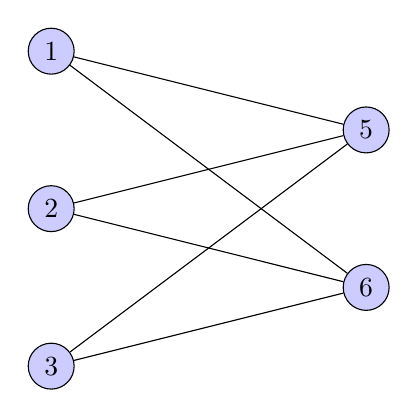
\begin{tikzpicture}[main_node/.style={circle,fill=blue!20,draw,minimum size=1em,inner sep=3pt]}]
		
		\node[main_node] (3) at (0,2) {3};
		\node[main_node] (2) at (0,4) {2};
		\node[main_node] (1) at (0,6) {1};
		\node[main_node] (5) at (4,3) {6};
		\node[main_node] (4) at (4,5) {5};
		

		\draw (1) -- (4);
		\draw (2) -- (4);
		\draw (3) -- (4);
		\draw (1) -- (5);
		\draw (2) -- (5);
		\draw (3) -- (5);
		\end{tikzpicture}
	\end{center}
	\caption{$K_{3,2}$}
	\label{K3,2}
\end{figure}
after 1 iteration of strategy S we get,
\begin{figure}[H]
	\begin{center}
		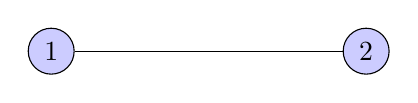
\begin{tikzpicture}[main_node/.style={circle,fill=blue!20,draw,minimum size=1em,inner sep=3pt]}]

		\node[main_node] (1) at (0,0) {1};
		\node[main_node] (2) at (4,0) {2};


		\draw (1) -- (2);
		\end{tikzpicture}
	\end{center}
	\caption{$K_{1,1}$}
	\label{K1,1}
\end{figure}
we now have a situation where $i = j$, so the KO-number for $K_{3,2}$ is 2.
\subsubsection{}
Reducing $K_{3,3}$ using strategy S,
\begin{figure}[H]
	\begin{center}
		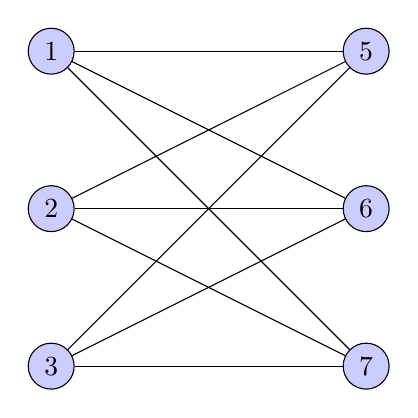
\begin{tikzpicture}[main_node/.style={circle,fill=blue!20,draw,minimum size=1em,inner sep=3pt]}]
		
		\node[main_node] (3) at (0,2) {3};
		\node[main_node] (2) at (0,4) {2};
		\node[main_node] (1) at (0,6) {1};
		\node[main_node] (6) at (4,2) {7};
		\node[main_node] (5) at (4,4) {6};
		\node[main_node] (4) at (4,6) {5};
		

		\draw (1) -- (4);
		\draw (2) -- (4);
		\draw (3) -- (4);
		\draw (1) -- (5);
		\draw (2) -- (5);
		\draw (3) -- (5);
		\draw (1) -- (6);
		\draw (2) -- (6);
		\draw (3) -- (6);
		\end{tikzpicture}
	\end{center}
	\caption{$K_{3,3}$}
	\label{K3,3}
\end{figure}
we have a situation where $i =j$, so the KO-number for $K_{3,3}$ is 1.
\subsubsection{}
Reducing $K_{3,4}$, using strategy S,
\begin{figure}[H]
	\begin{center}
		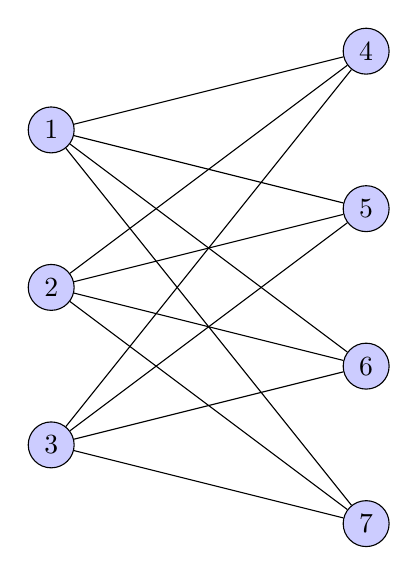
\begin{tikzpicture}[main_node/.style={circle,fill=blue!20,draw,minimum size=1em,inner sep=3pt]}]
		
		\node[main_node] (3) at (0,2) {3};
		\node[main_node] (2) at (0,4) {2};
		\node[main_node] (1) at (0,6) {1};
		\node[main_node] (7) at (4,1) {7};
		\node[main_node] (6) at (4,3) {6};
		\node[main_node] (5) at (4,5) {5};
		\node[main_node] (4) at (4,7) {4};
		
		\draw (1) -- (4);
		\draw (2) -- (4);
		\draw (3) -- (4);
		\draw (1) -- (5);
		\draw (2) -- (5);
		\draw (3) -- (5);
		\draw (1) -- (6);
		\draw (2) -- (6);
		\draw (3) -- (6);
		\draw (1) -- (7);
		\draw (2) -- (7);
		\draw (3) -- (7);
		\end{tikzpicture}
	\end{center}
	\caption{$K_{3,4}$}
	\label{K3,4}
\end{figure}
after one iteration of S we get,
\begin{figure}[H]
	\begin{center}
		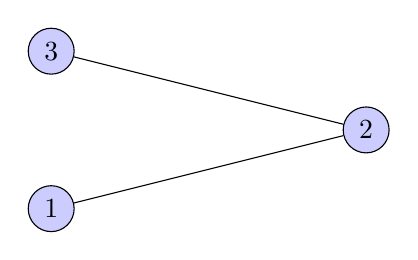
\begin{tikzpicture}[main_node/.style={circle,fill=blue!20,draw,minimum size=1em,inner sep=3pt]}]

		\node[main_node] (1) at (0,0) {1};
		\node[main_node] (3) at (0,2) {3};
		\node[main_node] (2) at (4,1) {2};


		\draw (2) -- (3);
		\draw (1) -- (2);
		\end{tikzpicture}
	\end{center}
	\caption{$P_{3}$}
	\label{P3}
\end{figure}
$P_{3}$ is clearly not KO-reducible, so we need to consider a smarter strategy.
We want to get a situation where $i =j$ after some KO-round. So, if each vertex in $V_{1}$ selects a different vertex in $V_{2}$ and 2 of the vertices in $V_{1}$ are selected by the vertices in $V_{2}$; we get,
\begin{figure}[H]
	\begin{center}
		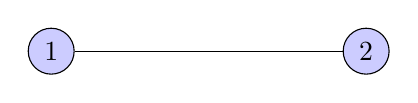
\begin{tikzpicture}[main_node/.style={circle,fill=blue!20,draw,minimum size=1em,inner sep=3pt]}]

		\node[main_node] (1) at (0,0) {1};
		\node[main_node] (2) at (4,0) {2};


		\draw (1) -- (2);
		\end{tikzpicture}
	\end{center}
	\caption{$K_{1,1}$}
	\label{K1,1}
\end{figure}
we now have a situation where $i =j$, so the KO-number for $K_{3,4}$ is 2.
\subsubsection{}
Reducing $K_{3,5}$, using strategy S,
\begin{figure}[H]
	\begin{center}
		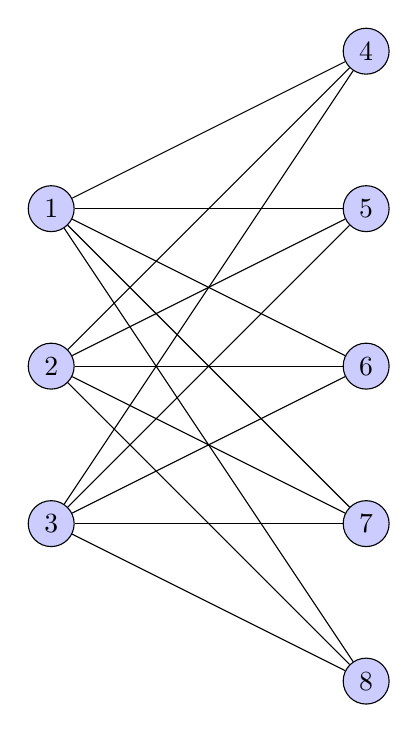
\begin{tikzpicture}[main_node/.style={circle,fill=blue!20,draw,minimum size=1em,inner sep=3pt]}]
		
		\node[main_node] (3) at (0,2) {3};
		\node[main_node] (2) at (0,4) {2};
		\node[main_node] (1) at (0,6) {1};
		\node[main_node] (8) at (4,0) {8};
		\node[main_node] (7) at (4,2) {7};
		\node[main_node] (6) at (4,4) {6};
		\node[main_node] (5) at (4,6) {5};
		\node[main_node] (4) at (4,8) {4};
		
		\draw (1) -- (4);
		\draw (2) -- (4);
		\draw (3) -- (4);
		\draw (1) -- (5);
		\draw (2) -- (5);
		\draw (3) -- (5);
		\draw (1) -- (6);
		\draw (2) -- (6);
		\draw (3) -- (6);
		\draw (1) -- (7);
		\draw (2) -- (7);
		\draw (3) -- (7);
		\draw (1) -- (8);
		\draw (2) -- (8);
		\draw (3) -- (8);
		\end{tikzpicture}
	\end{center}
	\caption{$K_{3,5}$}
	\label{K3,5}
\end{figure}
after one iteration of S we get,
\begin{figure}[H]
	\begin{center}
		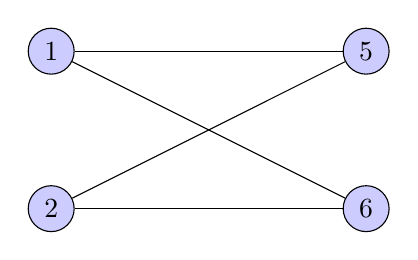
\begin{tikzpicture}[main_node/.style={circle,fill=blue!20,draw,minimum size=1em,inner sep=3pt]}]
		
		\node[main_node] (2) at (0,4) {2};
		\node[main_node] (1) at (0,6) {1};
		\node[main_node] (4) at (4,4) {6};
		\node[main_node] (3) at (4,6) {5};
		

		\draw (1) -- (3);
		\draw (2) -- (3);
		\draw (1) -- (4);
		\draw (2) -- (4);
		\end{tikzpicture}
	\end{center}
	\caption{$K_{2,2}$}
	\label{K2,2}
\end{figure}
we now have a situation where $i =j$, so the KO-number for $K_{3,5}$ is 2.
\subsubsection{}
Reducing $K_{3,6}$, using strategy S,
\begin{figure}[H]
	\begin{center}
		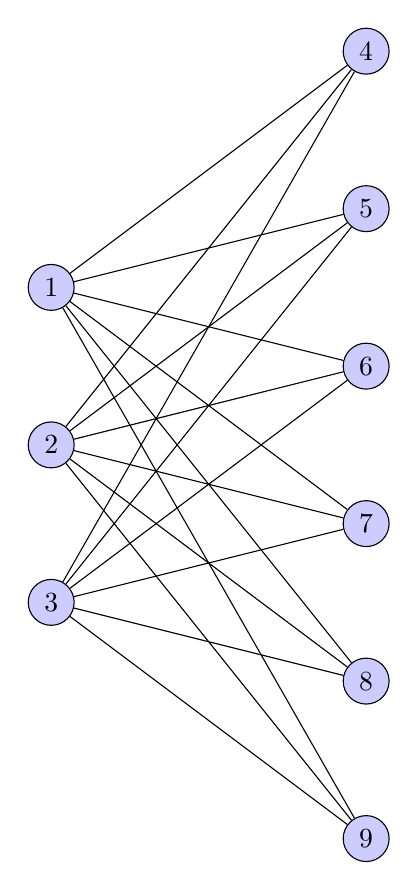
\begin{tikzpicture}[main_node/.style={circle,fill=blue!20,draw,minimum size=1em,inner sep=3pt]}]
		
		\node[main_node] (3) at (0,3) {3};
		\node[main_node] (2) at (0,5) {2};
		\node[main_node] (1) at (0,7) {1};
		\node[main_node] (9) at (4,0) {9};
		\node[main_node] (8) at (4,2) {8};
		\node[main_node] (7) at (4,4) {7};
		\node[main_node] (6) at (4,6) {6};
		\node[main_node] (5) at (4,8) {5};
		\node[main_node] (4) at (4,10) {4};
		
		\draw (1) -- (4);
		\draw (2) -- (4);
		\draw (3) -- (4);
		\draw (1) -- (5);
		\draw (2) -- (5);
		\draw (3) -- (5);
		\draw (1) -- (6);
		\draw (2) -- (6);
		\draw (3) -- (6);
		\draw (1) -- (7);
		\draw (2) -- (7);
		\draw (3) -- (7);
		\draw (1) -- (8);
		\draw (2) -- (8);
		\draw (3) -- (8);
		\draw (1) -- (9);
		\draw (2) -- (9);
		\draw (3) -- (9);
		\end{tikzpicture}
	\end{center}
	\caption{$K_{3,6}$}
	\label{K3,6}
\end{figure}
after one iteration of S we get,
\begin{figure}[H]
	\begin{center}
		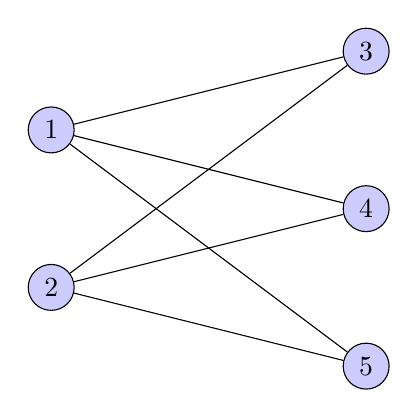
\begin{tikzpicture}[main_node/.style={circle,fill=blue!20,draw,minimum size=1em,inner sep=3pt]}]
		
		\node[main_node] (2) at (0,3) {2};
		\node[main_node] (1) at (0,5) {1};
		\node[main_node] (5) at (4,2) {5};
		\node[main_node] (4) at (4,4) {4};
		\node[main_node] (3) at (4,6) {3};
		

		\draw (3) -- (1);
		\draw (4) -- (1);
		\draw (5) -- (1);
		\draw (3) -- (2);
		\draw (4) -- (2);
		\draw (5) -- (2);
		\end{tikzpicture}
	\end{center}
	\caption{$K_{2,3}$}
	\label{K2,3}
\end{figure}
after another iteration of S we get,
\begin{figure}[H]
	\begin{center}
		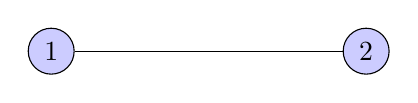
\begin{tikzpicture}[main_node/.style={circle,fill=blue!20,draw,minimum size=1em,inner sep=3pt]}]

		\node[main_node] (1) at (0,0) {1};
		\node[main_node] (2) at (4,0) {2};


		\draw (1) -- (2);
		\end{tikzpicture}
	\end{center}
	\caption{$K_{1,1}$}
	\label{K1,1}
\end{figure}
we now have a situation where $i =j$, so the KO-number for $K_{3,6}$ is 3.
\subsubsection{}
Reducing $K_{3,7}$, using strategy S,
\begin{figure}[H]
	\begin{center}
		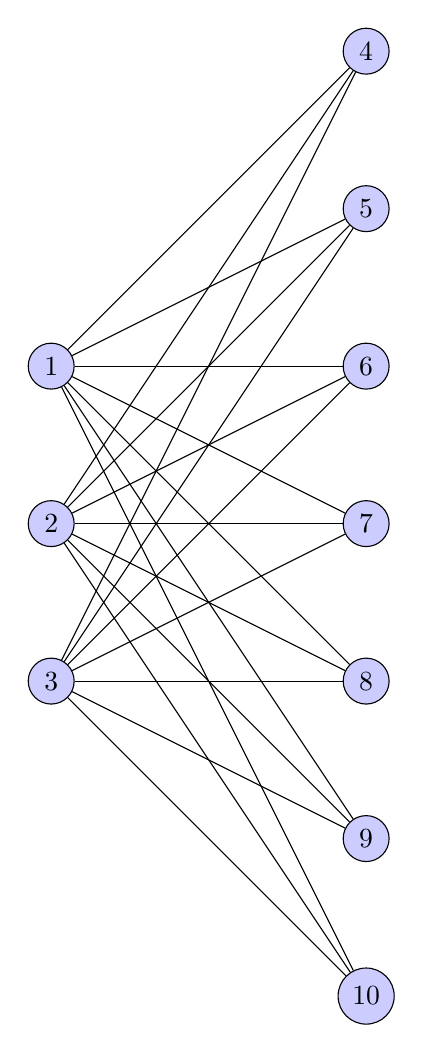
\begin{tikzpicture}[main_node/.style={circle,fill=blue!20,draw,minimum size=1em,inner sep=3pt]}]
		
		\node[main_node] (3) at (0,4) {3};
		\node[main_node] (2) at (0,6) {2};
		\node[main_node] (1) at (0,8) {1};
		\node[main_node] (10) at (4,0) {10};
		\node[main_node] (9) at (4,2) {9};
		\node[main_node] (8) at (4,4) {8};
		\node[main_node] (7) at (4,6) {7};
		\node[main_node] (6) at (4,8) {6};
		\node[main_node] (5) at (4,10) {5};
		\node[main_node] (4) at (4,12) {4};
		
		\draw (1) -- (4);
		\draw (2) -- (4);
		\draw (3) -- (4);
		\draw (1) -- (5);
		\draw (2) -- (5);
		\draw (3) -- (5);
		\draw (1) -- (6);
		\draw (2) -- (6);
		\draw (3) -- (6);
		\draw (1) -- (7);
		\draw (2) -- (7);
		\draw (3) -- (7);
		\draw (1) -- (8);
		\draw (2) -- (8);
		\draw (3) -- (8);
		\draw (1) -- (9);
		\draw (2) -- (9);
		\draw (3) -- (9);
		\draw (1) -- (10);
		\draw (2) -- (10);
		\draw (3) -- (10);
		\end{tikzpicture}
	\end{center}
	\caption{$K_{3,7}$}
	\label{K3,7}
\end{figure}
after one iteration of S we get,
\begin{figure}[H]
	\begin{center}
		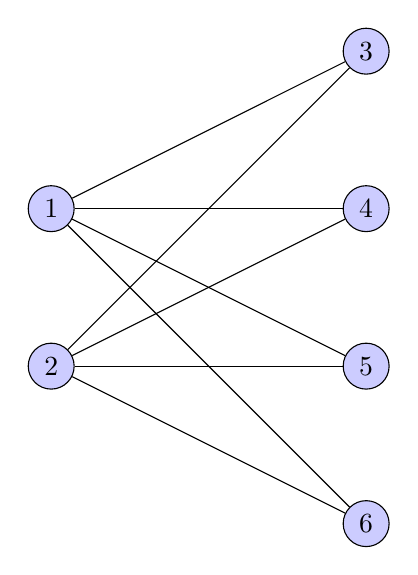
\begin{tikzpicture}[main_node/.style={circle,fill=blue!20,draw,minimum size=1em,inner sep=3pt]}]
		
		\node[main_node] (2) at (0,2) {2};
		\node[main_node] (1) at (0,4) {1};
		\node[main_node] (5) at (4,2) {5};
		\node[main_node] (4) at (4,4) {4};
		\node[main_node] (3) at (4,6) {3};
		\node[main_node] (6) at (4,0) {6};
		

		\draw (3) -- (1);
		\draw (4) -- (1);
		\draw (5) -- (1);
		\draw (6) -- (1);
		\draw (3) -- (2);
		\draw (4) -- (2);
		\draw (5) -- (2);
		\draw (6) -- (2);
		\end{tikzpicture}
	\end{center}
	\caption{$K_{2,4}$}
	\label{K2,4}
\end{figure}
after another iteration of S we get,
\begin{figure}[H]
	\begin{center}
		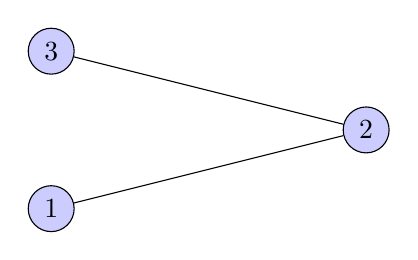
\begin{tikzpicture}[main_node/.style={circle,fill=blue!20,draw,minimum size=1em,inner sep=3pt]}]

		\node[main_node] (1) at (0,0) {1};
		\node[main_node] (3) at (0,2) {3};
		\node[main_node] (2) at (4,1) {2};


		\draw (2) -- (3);
		\draw (1) -- (2);
		\end{tikzpicture}
	\end{center}
	\caption{$P_{3}$}
	\label{P3}
\end{figure}
$P_{3}$ is clearly not KO-reducible, so $K_{3,7}$ is not KO-reducible. Actually for any $q \geq 7$, $K_{3,q}$ is not KO-reducible. Because, after we apply our strategy S to the graph $K_{3,q}$ where $q \geq 6$, we are always left with a star graph $S_{(q-5)}$. $S_{1}$ is KO-reducible because $S_{1} \equiv K_{1,1}$, which is an $i =j$ situtaion, which we know is KO-reducible, so for $q=6$, $K_{3,q}$ is KO-reducible. However, $S_{n}$ is clearly not KO-reducible for $n \geq 2$ (we will always get atleast one isolated vertex), so $K_{3,q}$ is not KO-reducible for $q \geq 7$ ($P_{3} \equiv S_{2}$).
\\
\\
So for all $k \geq 7$,
\begin{center}
\begin{tabular}{|c|c|}
	\hline
	Graph & KO-number	\\
	\hline
	$K_{3,2}$ & 2	\\
	\hline
	$K_{3,3}$ & 1	\\
	\hline
	$K_{3,4}$ & 2	\\
	\hline
	$K_{3,5}$ & 2	\\
	\hline
	$K_{3,6}$ & 3	\\
	\hline
	$K_{3,7}$ & $\infty$	\\
	\hline
	... & ...	\\
	\hline
	$K_{3,k}$ & $\infty$	\\
	\hline
\end{tabular}  
\end{center}
\newpage
\section{Logic and Discrete Structures}
\subsection{}
$\varphi = ((a \wedge b)\implies c) \wedge(a \vee b)$
\subsubsection{}
\begin{center}
\begin{tabular}{|c|c|c|cccccccccc|c|}
	\hline 
	a & b & c & ((a $\wedge$&b&)&$\implies$&c&)&$\wedge$&(a $\vee$&b&)& $\varphi$ \\ 
	\hline 
	T & T & T &T&T&T&&T&T&&T&T&T& T \\ 
	\hline 
	T & T & F &T&T&T&&F&F&&T&T&T&  F \\ 
	\hline 
	T & F & T &T&F&F&&T&T&&T&F&T& T  \\ 
	\hline 
	T & F & F &T&F&F&&F&T&&T&F&T& T \\ 
	\hline 
	F & T & T &F&T&F&&T&T&&F&T&T& T \\ 
	\hline 
	F & T & F &F&T&F&&F&T&&F&T&T& T  \\ 
	\hline 
	F & F & T &F&F&F&&T&T&&F&F&F& F  \\ 
	\hline 
	F & F & F &F&F&F&&F&T&&F&F&F&  F \\ 
	\hline 
\end{tabular} 
\end{center}
So in d.n.f, $\varphi = (a \wedge b \wedge c) \vee (a \wedge \neg b \wedge c) \vee (a \wedge \neg b \wedge \neg c) \vee (\neg a \wedge b \wedge c) \vee (\neg a \wedge b \wedge \neg c)$
\subsubsection{}
Negating $\varphi $ we get:
\\
$\neg \varphi$ = $\neg((a \wedge b \wedge c) \vee (a \wedge \neg b \wedge c) \vee (a \wedge \neg b \wedge \neg c) \vee (\neg a \wedge b \wedge c) \vee (\neg a \wedge b \wedge \neg c))$
\\
\\
by generalised de morgan's laws:
\\
$\neg \varphi$ = $\neg(a \wedge b \wedge c) \wedge \neg(a \wedge \neg b \wedge c) \wedge \neg(a \wedge \neg b \wedge \neg c) \wedge \neg(\neg a \wedge b \wedge c) \wedge \neg(\neg a \wedge b \wedge \neg c)$
\\
\\
by generalised de morgan's laws again we get $\neg \varphi$ in c.n.f:
\\
$\varphi = (\neg a \vee \neg b \vee \neg c) \wedge (\neg a\vee b \vee \neg c) \wedge (\neg a \vee b \vee c) \wedge (a \vee \neg b \vee \neg c) \wedge (a \vee \neg b \vee c)$

\subsection{}
We know the set $\{\neg , \wedge , \vee\}$ is a functionally complete set. To show the set $\{\wedge,\oplus\} $ is functionally complete we will try to construct logically equivalent statements of all the elements in the set $\{\neg , \wedge , \vee\}$ with elements of the set $\{\wedge,\oplus\} $
\\
\\
Obviously, $\wedge$ can be made from the set  $\{\wedge,\oplus\} $:
\\
$p \wedge q \equiv p \wedge q$
\\
\\
Making $\vee$:
\\
try $(p \oplus q) \oplus (p \wedge q)$,
\begin{center}
\begin{tabular}{|c|c|ccccccc|c|cc|c|}
	\hline 
	p & q & (p $ \oplus$ &q&)& $\oplus$ &(p $\wedge$ &q&)& $\varphi$ & p $\vee$ & q & $\Psi$ \\ 
	\hline 
	T & T & T & T & F& & T & & T & T & T & T & T \\ 
	\hline 
	T & F & T & F & T& & T & & F & T & T &  F & T \\ 
	\hline 
	F & T & F & T & T& & F & & T & T & F & T & T  \\ 
	\hline 
	F & F & F & F & F& & F & & F & F & F & F & F \\ 
	\hline 
\end{tabular} 
\end{center}
where $p\oplus q \equiv\neg (p\iff q)$.
\\
\\
$\varphi \equiv \Psi$, so $(p \oplus q) \oplus (p \wedge q) \equiv p \vee q$
\\
Therefore $\vee$ can be made from the set $\{\wedge,\oplus\} $, we can now use $\vee$ as an operator.
\\
\\
Making $\neg $:
\\
The operator $\neg$ has only one operand, so $\neg$ must be made from one operand p, using the elements from the set $\{\wedge,\oplus\}$, along with $\vee$ which we have just made.
\\
\\
$(p \oplus p)$ is always false, so we can use $F$ as an operand.
\\
$(p \wedge p)$ is always $p$.
\\
$(p \vee p)$ is always $p$.
\\
$(p \wedge F)$ is always False.
\\
$(p \vee F)$ is always $p$.
\\
$(p \oplus F) $is always $p$.
\\
\\
We can see the operator $\neg$ can't be made from the set $\{\wedge,\oplus\} $, because we are only getting $p$ or False, from the various configurations of operators on the variable p. Therefore $\{\wedge,\oplus\} $ is not a functionally complete set.
\subsection{}
\subsubsection{}
$\neg a \wedge b \wedge (a \wedge (b \implies c)) \vdash c \vee d$
\\
\begin{logicproof}{2}
	\neg a \land b \land (a \lor (b \implies c)) & premise
	\\
	\neg a \land b & $\wedge e$
	\\
	a \lor (b \implies c) & $\wedge e$ 
	\\
	\neg a & $\wedge e$ 
	\\
	b & $\wedge e$ 
	\\
	\begin{subproof}
	a & assume
	\\
	\bot & $\neg e$ 
	\\
	c \lor d & $\bot e$ 
	\end{subproof}
	\begin{subproof}
	b \implies c & assume
	\\
	c & $\implies e$ 
	\\
	c \lor d & $\vee i$ 
	\end{subproof}
	c \lor d & $\vee e$ 
\end{logicproof}
\subsubsection{}
$a \vee(\neg b \wedge \neg c \wedge \neg d) \vdash (a \vee \neg b) \wedge (a \vee \neg c) \wedge (a \vee \neg d)$
\\
\begin{logicproof}{2}
	a \lor(\neg b \land \neg c \land \neg d) & premise
	\\
	\begin{subproof}
	a & assume
	\\
	a \lor \neg b & $\vee i$ 
	\end{subproof}
	\begin{subproof}
	\neg b \land \neg c \land \neg d & assume
	\\
	\neg b & $\wedge e$
	\\
	a \lor \neg b & $\vee i$ 
	\end{subproof}
	a \lor \neg b & $\vee e$ 
	\\
	\begin{subproof}
	a & assume
	\\
	a \lor \neg c & $\vee i$ 
	\end{subproof}
	\begin{subproof}
	\neg b \land \neg c \land \neg d & assume
	\\
	\neg c & $\wedge e$
	\\
	a \lor \neg c & $\vee i$ 
	\end{subproof}
	a \lor \neg c & $\vee e$ 
	\\
	\begin{subproof}
	a & assume
	\\
	a \lor \neg d & $\vee i$ 
	\end{subproof}
	\begin{subproof}
	\neg b \land \neg c \land \neg d & assume
	\\
	\neg d & $\wedge e$
	\\
	a \lor \neg d & $\vee i$ 
	\end{subproof}
	a \lor \neg d & $\vee e$ 
	\\
	(a \vee \neg b) \wedge (a \vee \neg c) & $\wedge i$
	\\
	(a \vee \neg b) \wedge (a \vee \neg c) \wedge (a \vee \neg d) & $\wedge i$
\end{logicproof}
\subsection{}
We negate $\varphi$ and put it in c.n.f, conveniently after $\varphi$ is negated $\neg \varphi$ is already in c.n.f so:
\\
\\
$\neg \varphi = a \wedge (\neg a \vee \neg b) \wedge (b \vee c) \wedge (\neg c \vee \neg d \vee e) \wedge (e \vee d) \wedge (\neg e \vee \neg c)$
\\
\\
Our set of clauses is:
\\
\\
$a, \neg a \vee \neg b, b \vee c, \neg c \vee \neg d \vee e, e \vee d, \neg e \vee \neg c$
\\
\\
Resolve on a, using: $a, \neg a \vee b$ to get a new set of clauses:
\\
\\
$\neg b, b \vee c, \neg c \vee \neg d \vee e, e \vee d, \neg e \vee \neg c$
\\
\\
Resolve on b, using: $\neg b, b \vee c$ to get a new set of clauses:
\\
\\
$c, \neg c \vee \neg d \vee e, e \vee d, \neg e \vee \neg c$
\\
\\
Resolve on c, using: $c, \neg c \vee \neg d \vee e$ to get a new set of clauses:
\\
\\
$\neg d \vee e, e \vee d, \neg e$
\\
\\
Resolve on e, using: $\neg d \vee e, e \vee d, \neg e$ to get a new set of clauses:
\\
\\
$\neg d, d$
\\
\\
From this we infer the empty clause $\varnothing$ so $\neg \varphi$ is a contradiction by resolution, and therefore $\varphi$ is a theorem.
\end{document}